\documentclass[a4paper]{article}

%% Language and font encodings
\usepackage[english]{babel}
\usepackage[utf8x]{inputenc}
\usepackage[T1]{fontenc}

%% Sets page size and margins
\usepackage[a4paper,top=3cm,bottom=2cm,left=3cm,right=3cm,marginparwidth=1.75cm]{geometry}

%% Useful packages
\usepackage{amsmath}
\usepackage{graphicx}
\usepackage{caption}
\usepackage{subcaption}
\usepackage[colorinlistoftodos]{todonotes}
\usepackage[colorlinks=true, allcolors=blue]{hyperref}

\title{Reporte de Actividad 7: Sistema de Resortes Acoplados}
\author{Jesús Antonio González Espinosa \\ \\ Física Computacional 1}
\date{Sábado, 24 de Marzo del 2018}

\begin{document}
\maketitle

\section{Introducción}

Para esta actividad hemos trabajado con modelación de fenómenos físicos en python; específicamente en el de oscilaciones, presentando varios ejemplos de sistemas de resortes acoplados.

En este reporte se continua trabajando con la síntesis del artículo "Coupled spring equations" de TEMPLE H. FAY, pero ahora con la adición de los últimos dos subtemas, el cual nos aporta la teoría necesaria para obtener las bases y comprender los conceptos importantes sobre sistemas de masas con oscilaciones no lineales y forzadas. Similarmente a la actividad pasada, el documento aporta ejemplos, presentando las propiedades y condiciones iniciales de los resortes para poder crear las gráficas presentadas en este reporte. Naturalmente, se presenta el cierre al reporte, incluyendo bilbiografía, conclusiones y el apéndice perteneciente a la actividad.


\section{Sintesis}
\subsection{Introducción}
En éste artículo se investiga el problema de los dos resortes y dos pesas adjuntas en serie. Bajo la suposición de que las fuerzas de restauración se comportan de acuerdo a la Ley de Hooke, este problema de dos grados de libertad es modelado por un par de ecuaciones diferenciales lineales de segundo orden que al sustituir una en la otra, el movimiento de cada pesa puede ser determinado por una ecuación diferencial lineal de cuarto orden. 

Lo que hace interesante a este problema, es que podemos investigar los movimientos de las masas, para ver si están sincronizadas u opuestas entre ellas. También se puede ver que al agregarle factores no lineares, pueden surgir movimientos interesantes. Al modificar los parámetros podemos observar gráficamente los cambios en la periodicidad, la amplitud, la fase, la sensitividad a loas condiciones iniciales, entre otras propiedades. 

\subsection{El modelo de resorte acoplado}
El modelo consiste en dos resortes y dos pesas. Un resorte tiene la constante elástica $k_1$ y está adjunto al techo de un extremo y del otro tiene una pesa de masa $m_1$. La misma pesa tiene adjunto un segundo resorte de constante elástica $k_2$ y al final de éste, una pesa de masa $m_2$. Al dejar el sistema llegar al equilibrio, medimos el desplazamiento de cada masa, en función del tiempo, y llamaremos estas medidas como: $x_1(t)$ y $x_2(t)$.

\begin{figure}[h]
 \centering
  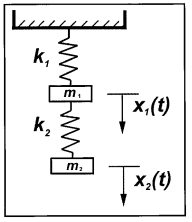
\includegraphics[width=0.2\textwidth]{ModeloResorte.PNG}
\end{figure}

\subsubsection{Asumiendo la Ley de Hooke}
Asumiendo que hay pequeñas oscilaciones, las fuerzas restauradoras son de la forma $- k_1l_1$ y $- k_2l_2$, donde $l_1$ y $l_2$ son las elongaciones o compresiones de los dos resortes. Como la masa superior está unida a ambos resortes, ésta siente las dos fuerzas restauradoras actuando sobre ella, mientras que la segunda masa solo siente la fuerza restauradora del segundo resorte. Asumiendo que no hay fuerzas de amortiguamiento, la Ley de Newton implica que las ecuaciones que representan los movimientos de las pesas son:

\begin{center}
$m_1\ddot x_1 = - k_1x_1 - k_2(x_1 - x_2)$

$m_1\ddot x_2 = - k_2(x_1 - x_2)$
\end{center}

Entonces para encontrar una ecuación para $x_1$ que no involucre a $x_2$, resolvemos la primera ecuación diferencial para $x_2$, y la sustituimos en la primera, donde después de simplificar, obtenemos:

\begin{center}
$m_1m_2x_1^{(4)} + (m_2k_1 + k_2(m_1 + m_2))\ddot x_1 + k_1k_2x_1 = 0$
\end{center}

Ahora, para encontrar una ecuación que involucre de $x_2$, resolvemos la segunda ecuación diferencial para $x_1$ y lo sustituimos en la primera ecuación, obteniendo:

\begin{center}
$m_1m_2x_2^{(4)} + (m_2k_1 + k_2(m_1 + m_2))\ddot x_1 + k_1k_2x_2 = 0$
\end{center}

Para poder resolver las ecuaciones, solo es necesario las posiciones iniciales y las velocidades iniciales.

\subsubsection{Algunos ejemplos con masas idénticas}
Consideremos el modelo con dos pesas con la misma masa, $m_1 = m_2 = 1$, ignorando el amortiguamiento y sin fuerzas externas.

\textbf{Ejemplo 2.1:} Describe el movimiento para las constantes de resorte $k_1 = 6$ y $k_2 = 4$ con las condiciones iniciales ($x_1(0), \dot x_1(0), x_2(0), \dot x_2(0)) = (1,0,2,0)$.
Al resolverlo de manera analítica obtenemos:
\begin{center}
$x_1(t) = cos \sqrt{2}t$

$x_2(t) = 2 cos \sqrt{2}t$
\end{center}

El movimiento es sincronizado, por lo tanto, las pesas se mueven en fase una con la otra, teniendo el mismo periodo, pero con amplitudes un poco diferentes. 

Para poder grafciar esto en Python, utilizamos un código proporcionado. Este código se utilizó durante toda la actividad, solo modificando los parámetros y condiciones iniciales; así como las variables de los ejes coordenados para presentar las diferentes gráficas. En este caso, el código para este ejemplo se ve así:

\begin{figure}[ht!]
 \centering
  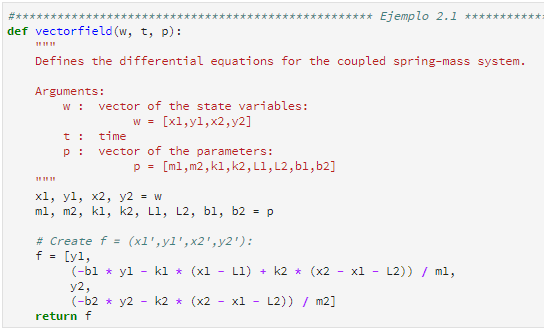
\includegraphics[width=0.65\textwidth]{Codigo1.PNG}
\end{figure}
\pagebreak
\begin{figure}[ht!]
 \centering
  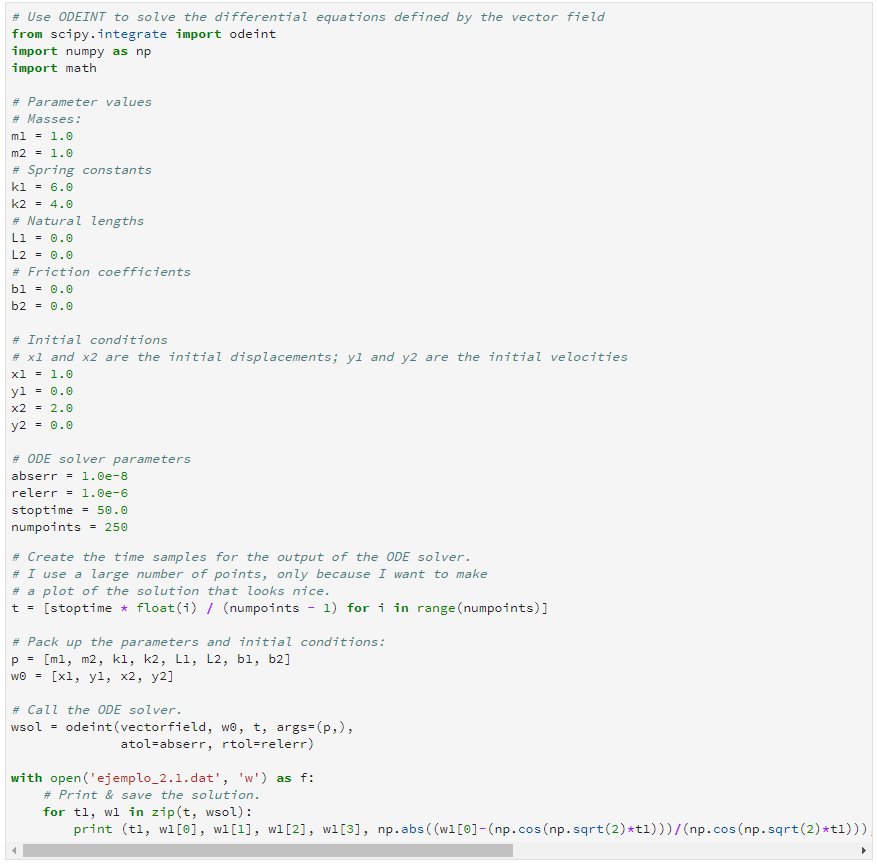
\includegraphics[width=0.65\textwidth]{Codigo2.PNG}
\end{figure}
\begin{figure}[ht!]
 \centering
  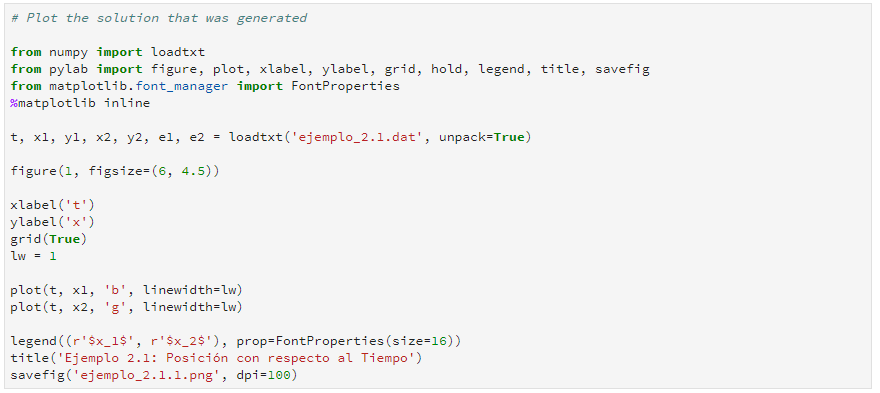
\includegraphics[width=0.65\textwidth]{Codigo3.PNG}
\end{figure}
Obteniendo las siguientes gráficas:
\begin{figure}[h!]
 \centering
  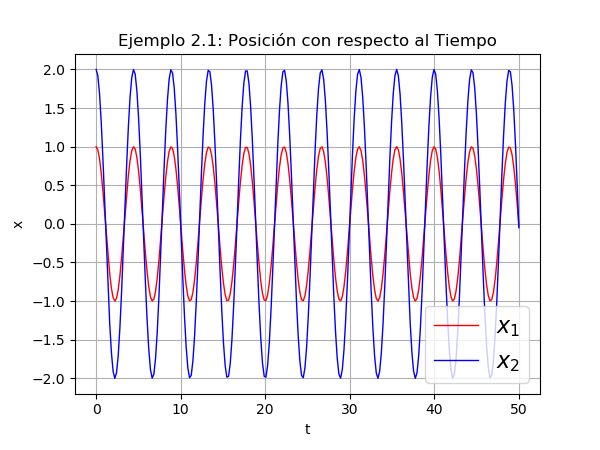
\includegraphics[width=0.65\textwidth]{ejemplo_2_1_1.png}
  \caption{Posición con respecto al Tiempo de $x_1$ y $x_2$}
\end{figure}

\pagebreak
\begin{figure}[ht!]
\begin{subfigure}{0.6\textwidth}
  \centering
  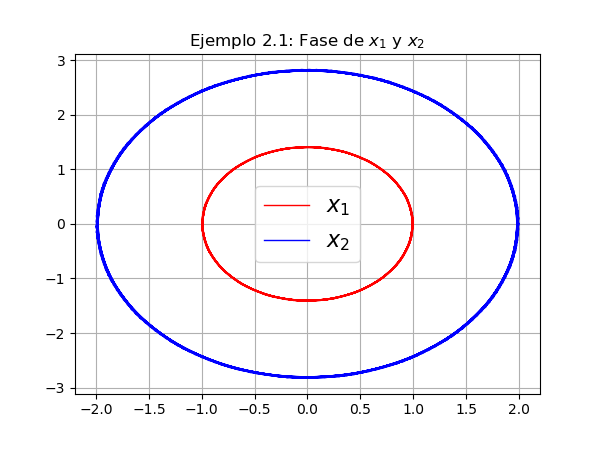
\includegraphics[width=\linewidth]{ejemplo_2_1_3.png}
   \caption{Fase de $x_1$ y $x_2$}
\end{subfigure}
\begin{subfigure}{0.6\textwidth}
  \centering
  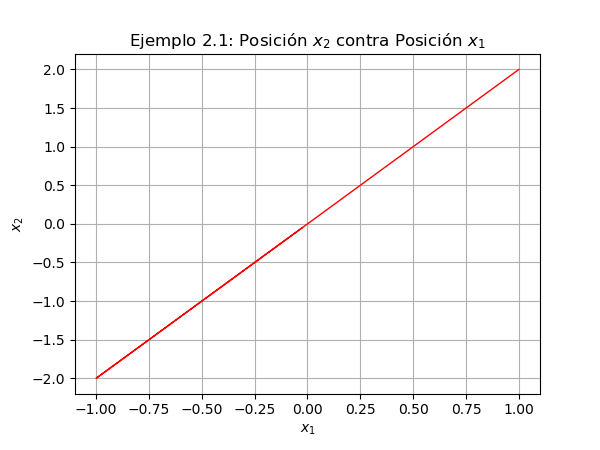
\includegraphics[width=\linewidth]{ejemplo_2_1_2.png}
  \caption{Posición $X_2$ contra $x_1$}
\end{subfigure}
\end{figure}

El error relativo de $x_1$ y $x_2$:

\begin{figure}[ht!]
\begin{subfigure}{0.6\textwidth}
  \centering
  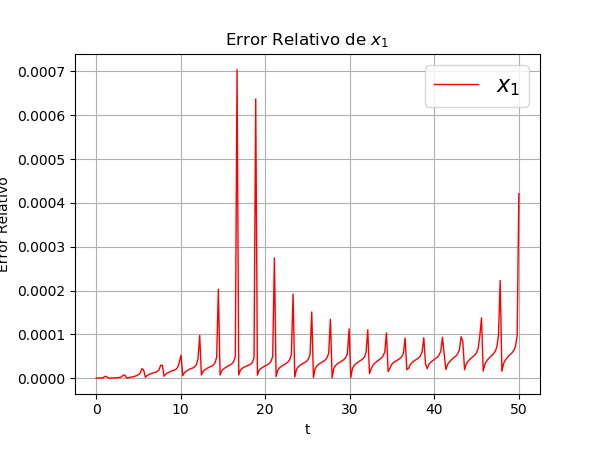
\includegraphics[width=\linewidth]{error2_1_1.png}
   \caption{Error Relativo de $x_1$}
\end{subfigure}
\begin{subfigure}{0.6\textwidth}
  \centering
  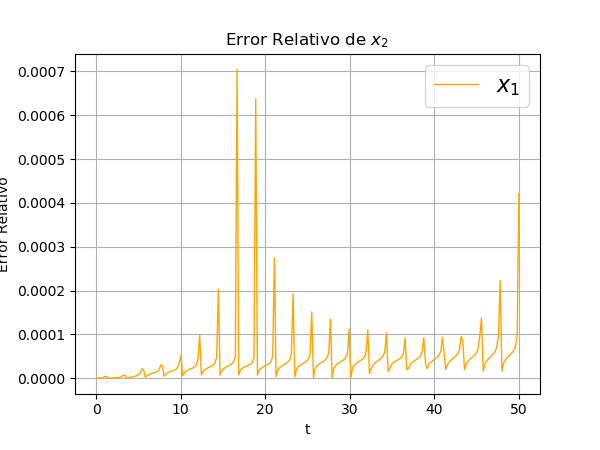
\includegraphics[width=\linewidth]{error2_1_2.png}
  \caption{Error Relativo de $x_2$}
\end{subfigure}
\end{figure}

\bigskip

\textbf{Ejemplo 2.2:} Describe el movimiento para las constantes de resorte $k_1 = 6$ y $k_2 = 4$ con las condiciones iniciales ($x_1(0), \dot x_1(0), x_2(0), \dot x_2(0)) = (-2,0,1,0)$.
Al resolverlo de manera analítica obtenemos:
\begin{center}
$x_1(t) = -2 cos 2\sqrt{3}t$

$x_2(t) = cos 2\sqrt{3}t$
\end{center}

En este caso, cuando la primera pesa se mueve hacia arriba, la segunda se mueve hacia abajo; aún tienen el mismo periodo, pero ahora un desfase de $180^\circ$

El código modificado para hacer tales gráficas resulta así:

\begin{figure}[ht!]
 \centering
  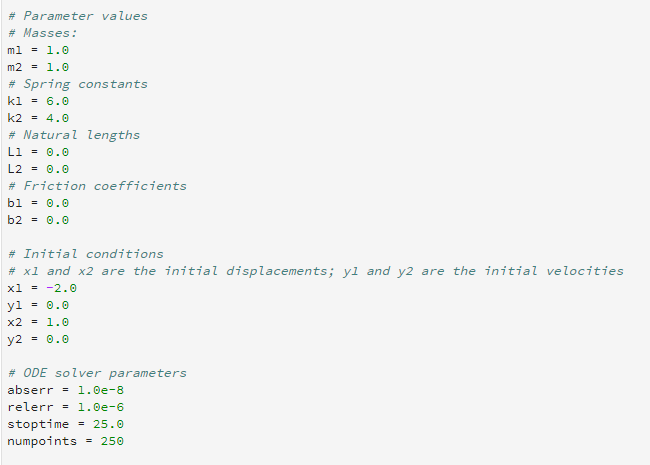
\includegraphics[width=0.65\textwidth]{Codigo2_1.PNG}
\end{figure}

Obteniendo las siguientes gráficas:
\pagebreak

\begin{figure}[ht!]
\begin{subfigure}{0.6\textwidth}
  \centering
  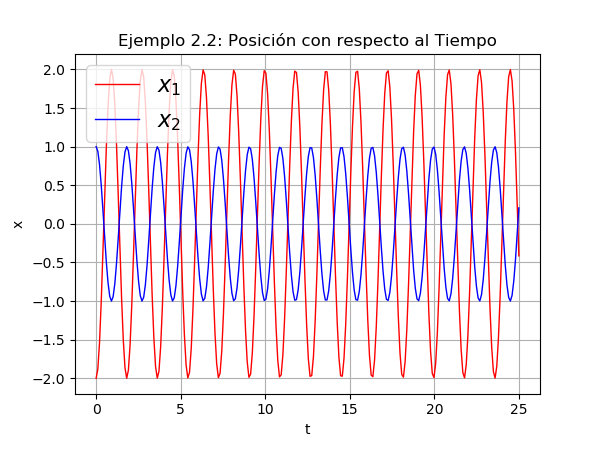
\includegraphics[width=\linewidth]{ejemplo_2_2_1.png}
   \caption{Posición con respecto al Tiempo de $x_1$ y $x_2$}
\end{subfigure}
\begin{subfigure}{0.6\textwidth}
  \centering
  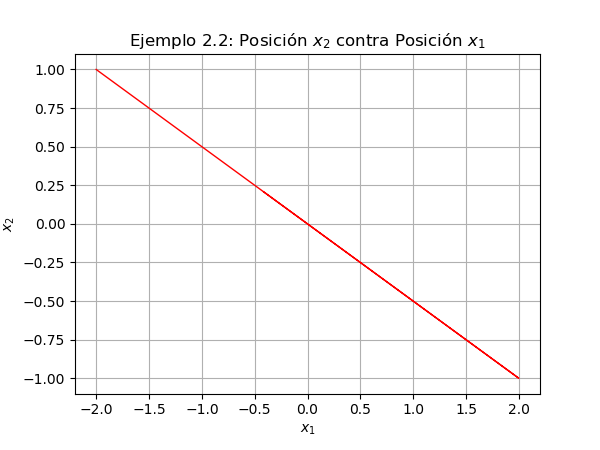
\includegraphics[width=\linewidth]{ejemplo_2_2_2.png}
  \caption{Posición $x_2$ contra $x_1$}
\end{subfigure}
\end{figure}

El error relativo de $x_1$ y $x_2$:

\begin{figure}[ht!]
\begin{subfigure}{0.6\textwidth}
  \centering
  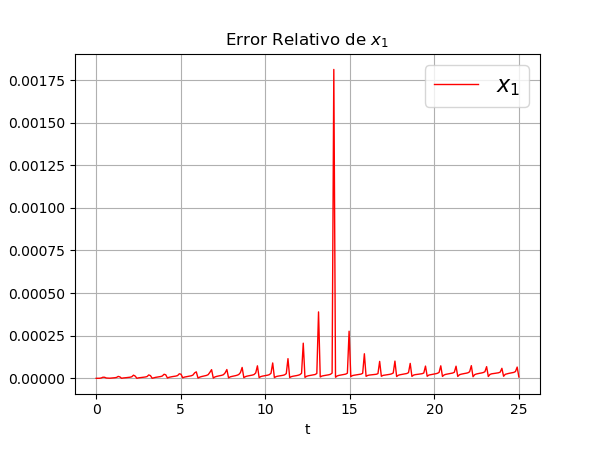
\includegraphics[width=\linewidth]{error2_2_1.png}
   \caption{Error Relativo de $x_1$}
\end{subfigure}
\begin{subfigure}{0.6\textwidth}
  \centering
  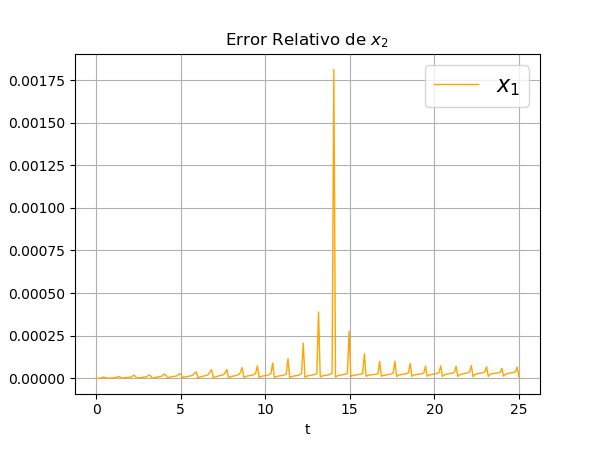
\includegraphics[width=\linewidth]{error2_2_2.png}
  \caption{Error Relativo de $x_2$}
\end{subfigure}
\end{figure}

\textbf{Ejemplo 2.3:} Describe el movimiento para las constantes de resorte $k_1 = 0.4$ y $k_2 = 1.808$ con las condiciones iniciales ($x_1(0), \dot x_1(0), x_2(0), \dot x_2(0)) = (1/2,0,-1/2,7/10)$.

En este problema, los valores de las constantes del resorte determinan el periodo y por lo tanto, la frecuencia; mientras que las condiciones iniciales solo afectan la amplitud y la fase de las soluciones. El código modificado para hacer tales gráficas resulta así:

\begin{figure}[ht!]
 \centering
  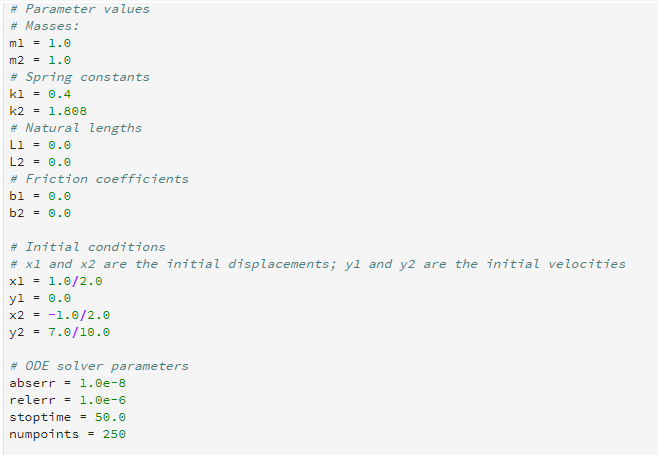
\includegraphics[width=0.65\textwidth]{Codigo2_2.PNG}
\end{figure}
 
Al graficar las soluciones, podemos ver varios patrones interesantes:

\begin{figure}[ht!]
\begin{subfigure}{0.6\textwidth}
  \centering
  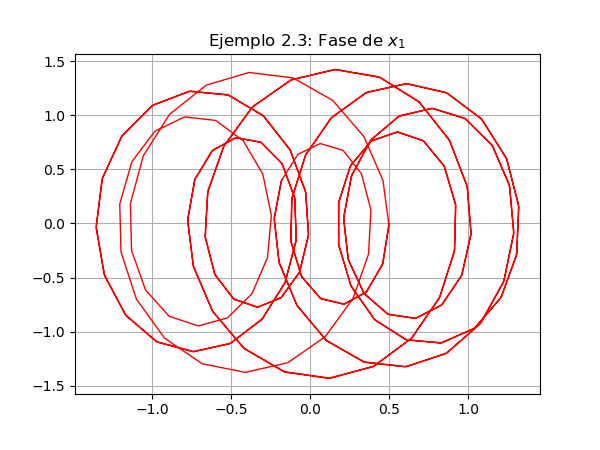
\includegraphics[width=\linewidth]{ejemplo_2_3_5.png}
   \caption{Fase para $x_1$}
\end{subfigure}
\begin{subfigure}{0.6\textwidth}
  \centering
  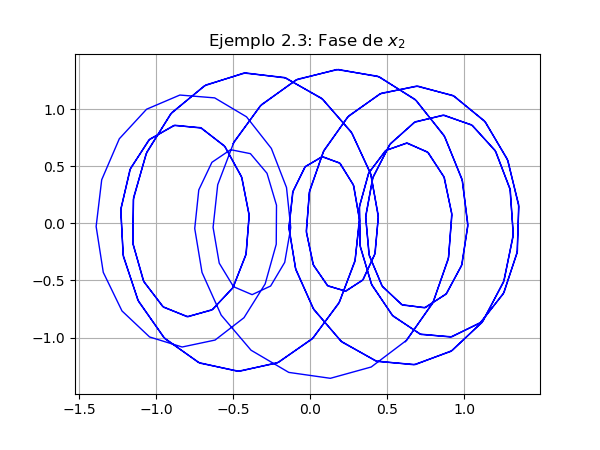
\includegraphics[width=\linewidth]{ejemplo_2_3_6.png}
  \caption{Fase para $x_2$}
\end{subfigure}
\begin{subfigure}{0.6\textwidth}
  \centering
  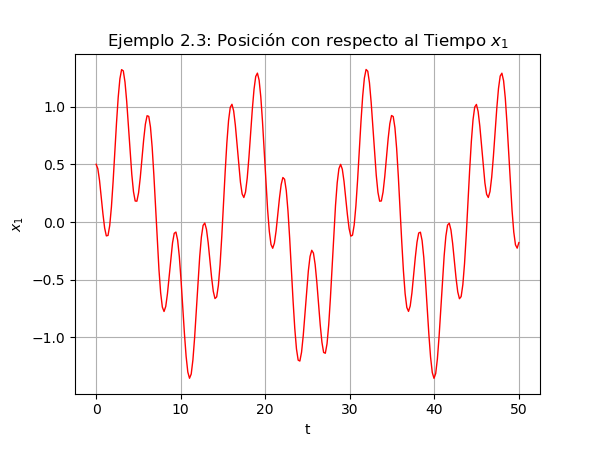
\includegraphics[width=\linewidth]{ejemplo_2_3_2.png}
  \caption{Posición con respecto al tiempo de $x_1$}
\end{subfigure}
\begin{subfigure}{0.6\textwidth}
  \centering
  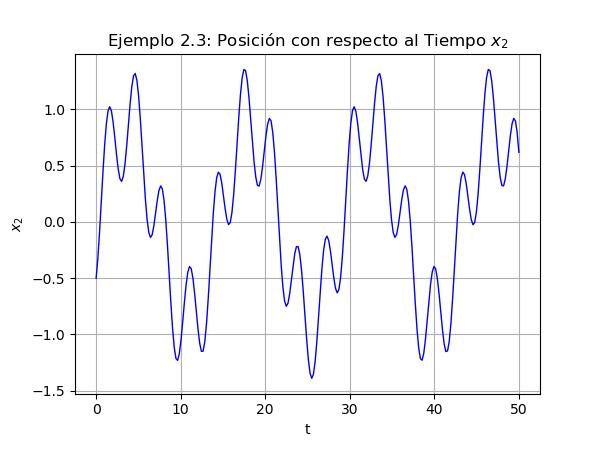
\includegraphics[width=\linewidth]{ejemplo_2_3_3.png}
  \caption{Posición con respecto al tiempo de $x_2$}
\end{subfigure}
\end{figure}
\begin{figure}[ht!]
\begin{subfigure}{0.6\textwidth}
  \centering
  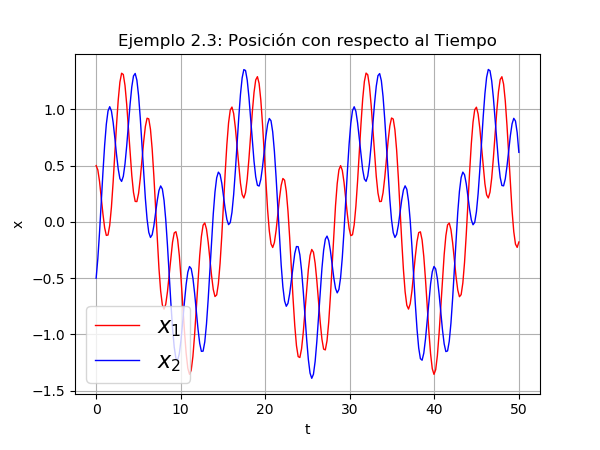
\includegraphics[width=\linewidth]{ejemplo_2_3_1.png}
  \caption{Posición con respecto al tiempo de $x_1$ y $x_2$}
\end{subfigure}
\begin{subfigure}{0.6\textwidth}
  \centering
  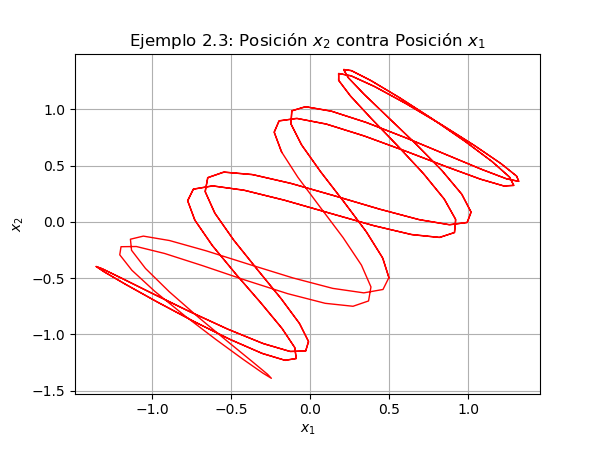
\includegraphics[width=\linewidth]{ejemplo_2_3_4.png}
  \caption{Posición $x_2$ contra $x_1$}
\end{subfigure}
\end{figure}

\subsubsection{Amortiguamiento}
El tipo de amortiguamiento más común, son los de viscosidad, donde la fuerza amortiguadora es proporcional a la velocidad. El amortiguamiento de la primera masa depende solamente de su velocidad y no de la velocidad de la segunda masa y vice versa. Para modelar esto, agregamos los términos $-\delta_1\dot x_1$ a la primera ecuación y $-\delta_1\dot x_2$ a la segunda. Asumiendo que los coeficientes de amortiguamiento $\delta_1$ y $\delta_2$ son pequeños, el modelo se da por:

\begin{center}
$m_1\ddot x_1 = - \delta_1\dot x_1 - k_1x_1 - k_2(x_1 - x_2)$

$m_2 \ddot x_2 = - \delta\dot x_2 - k_2(x_2 - x_1)$
\end{center}

Ahora, para hacer una ecuación que solo dependa de $x_2$, podemos resolver la segunda ecuación para $x_1$ y sustituirlo en la primera, obteniendo una ecuación de cuarto orden:

\begin{center}
$m_1m_2x_2^{(4)} + (m_1\delta_1 + m_2\delta_2)\dddot x_2 + (m_2k_1 + k_2(m_1 + m_2) + \delta_1\delta_2)\ddot x_2 + (k_1\delta_2 + k_2(\delta_1 + \delta_2)\dot x_2 + k_1k_2x_2 = 0$

Podemos hacer el mismo procedimiento para que dependa de $x_1$. Con esto, obtenemos una ecuación diferencial lineal que representa el movimiento de ambas pesas. 

\textbf{Ejemplo 2.4:} Asuma que $m_1 = m_2 = 1$. Describe el movimiento para las constantes de resorte $k_1 = 0.4$ y $k_2 = 1.808$, los coeficientes de amortiguamiento $\delta_1 = 0.1$ y $\delta_2 = 0.2$ con las condiciones iniciales ($x_1(0), \dot x_1(0), x_2(0), \dot x_2(0)) = (1,1/2,2,1/2)$.

Se puede observar un patrón regular en donde el movimiento avanza con una disminución en su amplitud. El código para graficar las soluciones resulta así:

\begin{figure}[ht!]
 \centering
  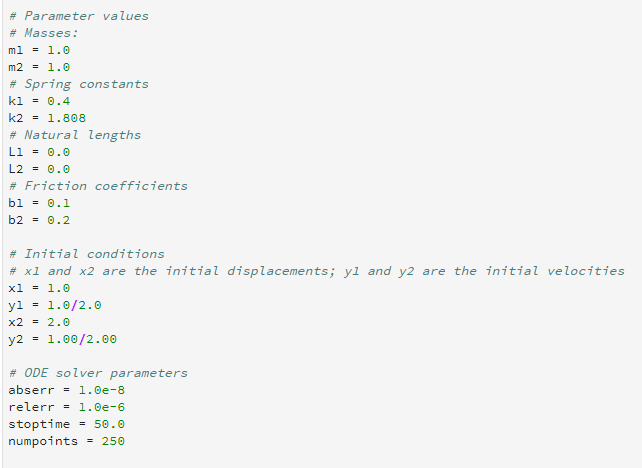
\includegraphics[width=0.65\textwidth]{Codigo2_3.PNG}
\end{figure}
 
\pagebreak

\raggedright Resultando en las siguientes graficas

\begin{figure}[ht!]
\begin{subfigure}{0.6\textwidth}
  \centering
  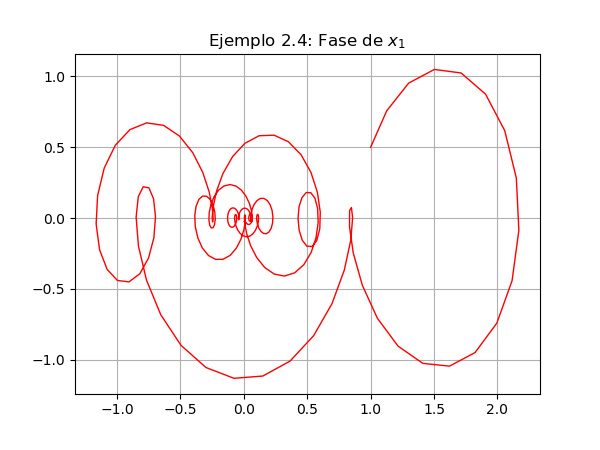
\includegraphics[width=\linewidth]{ejemplo_2_4_5.png}
   \caption{Fase para $x_1$}
\end{subfigure}
\begin{subfigure}{0.6\textwidth}
  \centering
  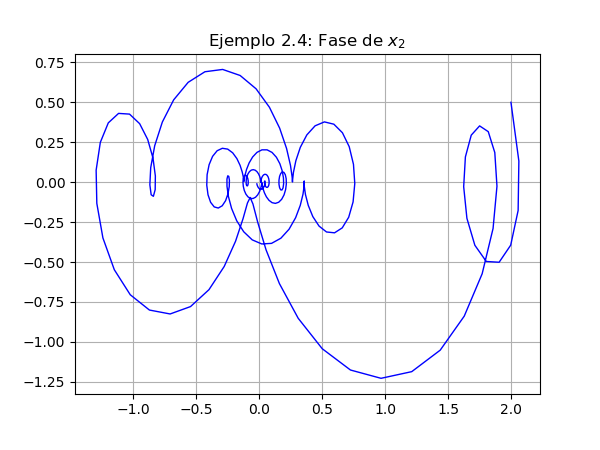
\includegraphics[width=\linewidth]{ejemplo_2_4_6.png}
  \caption{Fase para $x_2$}
\end{subfigure}
\begin{subfigure}{0.6\textwidth}
  \centering
  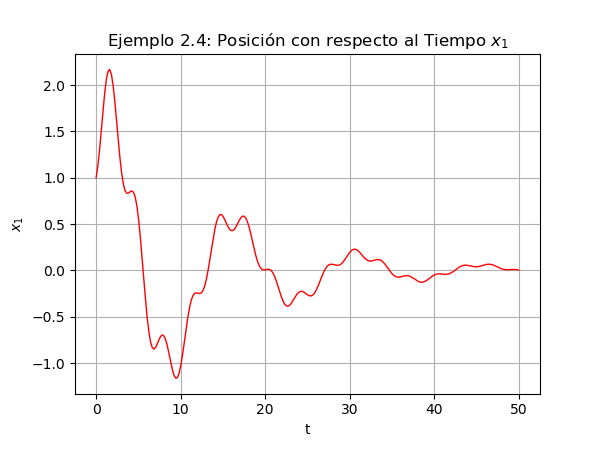
\includegraphics[width=\linewidth]{ejemplo_2_4_2.png}
  \caption{Posición con respecto al tiempo de $x_1$}
\end{subfigure}
\begin{subfigure}{0.6\textwidth}
  \centering
  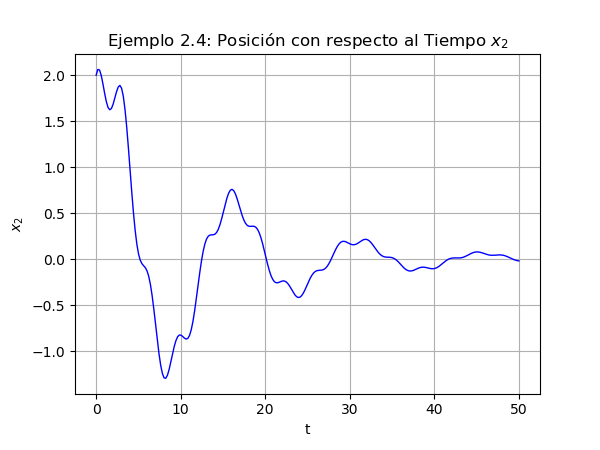
\includegraphics[width=\linewidth]{ejemplo_2_4_3.png}
  \caption{Posición con respecto al tiempo de $x_2$}
\end{subfigure}
\begin{subfigure}{0.6\textwidth}
  \centering
  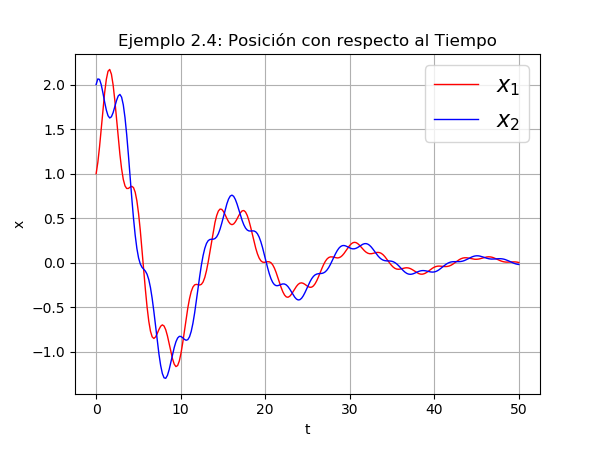
\includegraphics[width=\linewidth]{ejemplo_2_4_1.png}
  \caption{Posición con respecto al tiempo de $x_1$ y $x_2$}
\end{subfigure}
\begin{subfigure}{0.6\textwidth}
  \centering
  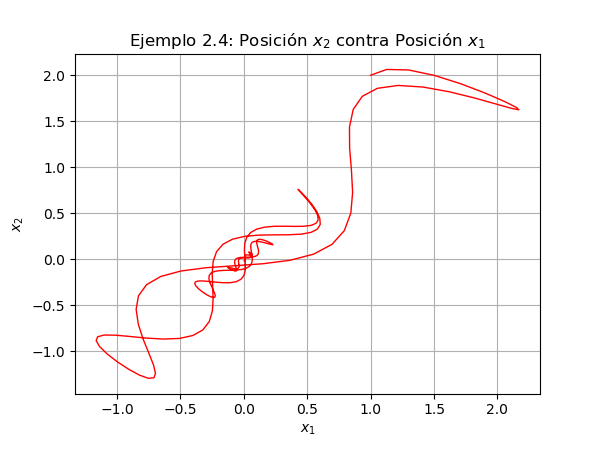
\includegraphics[width=\linewidth]{ejemplo_2_4_4.png}
  \caption{Posición $x_2$ contra $x_1$}
\end{subfigure}
\end{figure}

\subsection{Agregando No Linealidad}
Si asumimos que las fuerzas restauradoras son no lineales, podemos acomodar el modelo para que encaje a esto. Asumiendo que la fuerza restauradora tienen la forma de $-kx + \mu x^3$. Entonces el modelo se convierte en:
\begin{center}
$m_1\ddot x_1 = - \delta_1\dot x_1 - k_1x_1 + \mu_1x_1^3 - k_2(x_1 - x_2) + \mu_2(x_1 - x_2)^3$

$m_2 \ddot x_2 = - \delta\dot x_2 - k_2(x_2 - x_1) + \mu_2(x_2 - x_1)^3$
\end{center}

Los rangos de movimiento para los modelos no lineales son mucho más complicados que los lineales; la exactitud cada vez se vuelve más cuestionable al resolver las ecuaciones, no hay solución numérica que se mantenga precisa.

\smallskip
\textbf{Ejemplo 3.1:} Asuma que $m_1 = m_2 = 1$. Describe el movimiento para las constantes de resorte $k_1 = 0.4$ y $k_2 = 1.808$, los coeficientes de amortiguamiento $\delta_1 = 0$ y $\delta_2 = 0$, coeficientes no lineales $\mu_1 = -1/6$ y $\mu_2 = -1/10$ con las condiciones iniciales ($x_1(0), \dot x_1(0), x_2(0), \dot x_2(0)) = (1,0,-1/2,0)$.

En este ejemplo no hay amortiguamiento, entonces los movimientos parecen ser periódicos. Por la no linealidad, el modelo puede mostrar sensitividad a las condiciones iniciales.
\smallskip

Para poder graficar esto, tenemos que retomar el código que hemos estado utilizando, pero con unas modificaciones para poder agregar la no linealidad. Después de los cambios, el código resulta así:
\begin{figure}[ht!]
 \centering
  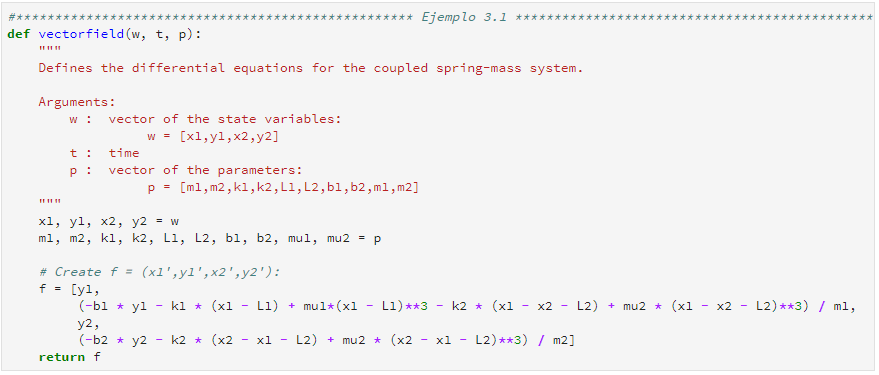
\includegraphics[width=0.65\textwidth]{Codigo4.PNG}
\end{figure}
\begin{figure}[ht!]
 \centering
  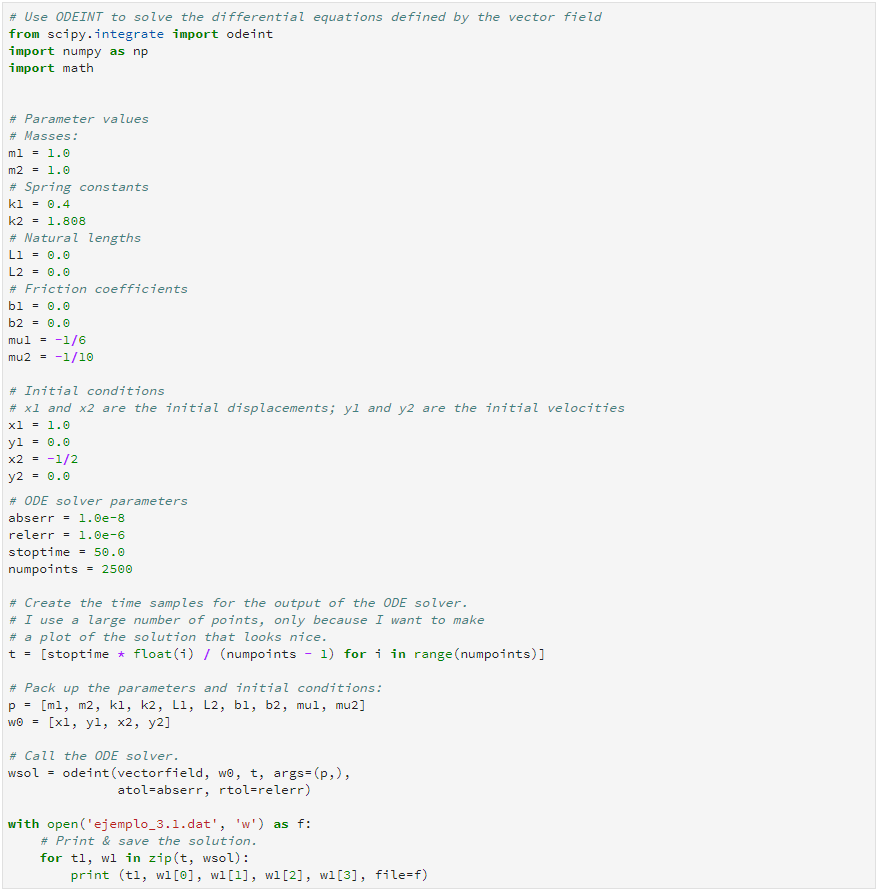
\includegraphics[width=0.65\textwidth]{Codigo5.png}
\end{figure}

\pagebreak

Y similarmente a los ejemplos anteriores, graficamos, obteniendo los siguientes resultados:

\begin{figure}[ht!]
\begin{subfigure}{0.6\textwidth}
  \centering
  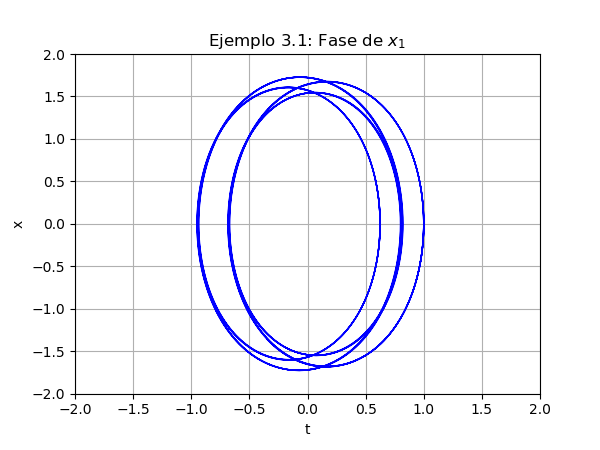
\includegraphics[width=\linewidth]{ejemplo_3_1_5.png}
   \caption{Fase para $x_1$}
\end{subfigure}
\begin{subfigure}{0.6\textwidth}
  \centering
  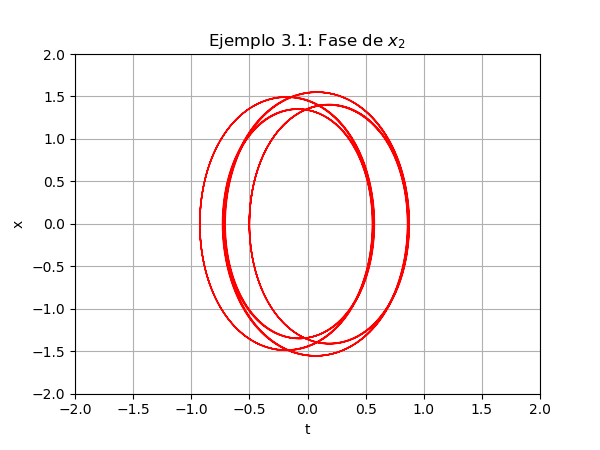
\includegraphics[width=\linewidth]{ejemplo_3_1_6.png}
  \caption{Fase para $x_2$}
\end{subfigure}
\begin{subfigure}{0.6\textwidth}
  \centering
  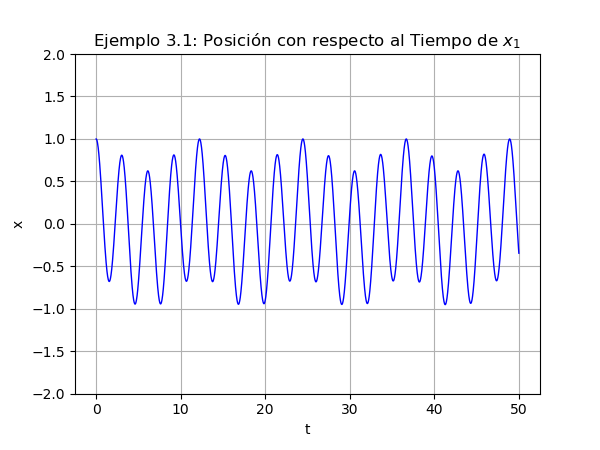
\includegraphics[width=\linewidth]{ejemplo_3_1_2.png}
  \caption{Posición con respecto al tiempo de $x_1$}
\end{subfigure}
\begin{subfigure}{0.6\textwidth}
  \centering
  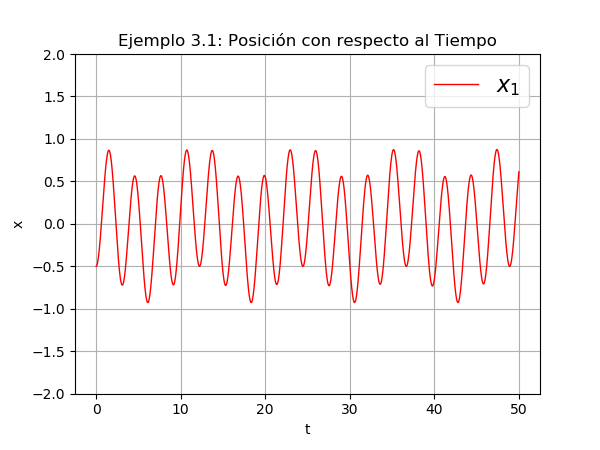
\includegraphics[width=\linewidth]{ejemplo_3_1_3.png}
  \caption{Posición con respecto al tiempo de $x_2$}
\end{subfigure}
\end{figure}
\begin{figure}[ht!]
\begin{subfigure}{0.6\textwidth}
  \centering
  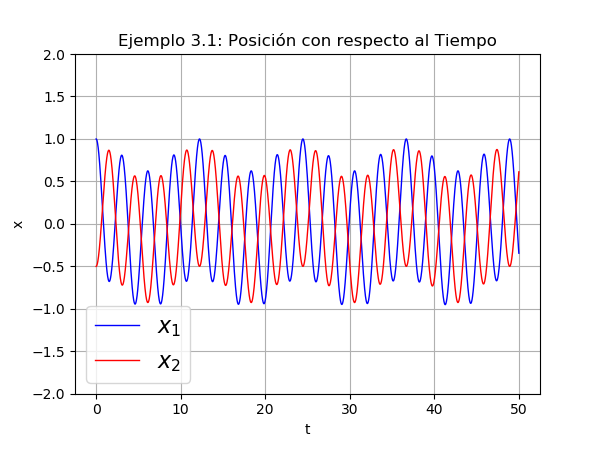
\includegraphics[width=\linewidth]{ejemplo_3_1_1.png}
  \caption{Posición con respecto al tiempo de $x_1$ y $x_2$}
\end{subfigure}
\begin{subfigure}{0.6\textwidth}
  \centering
  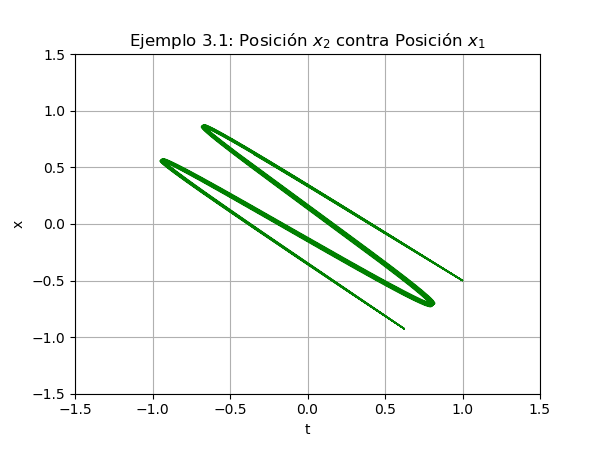
\includegraphics[width=\linewidth]{ejemplo_3_1_4.png}
  \caption{Posición $x_2$ contra $x_1$}
\end{subfigure}
\end{figure}

\pagebreak

\textbf{Ejemplo 3.2:} Asuma que $m_1 = m_2 = 1$. Describe el movimiento para las constantes de resorte $k_1 = 0.4$ y $k_2 = 1.808$, los coeficientes de amortiguamiento $\delta_1 = 0$ y $\delta_2 = 0$, coeficientes no lineales $\mu_1 = -1/6$ y $\mu_2 = -1/10$ con las condiciones iniciales ($x_1(0), \dot x_1(0), x_2(0), \dot x_2(0)) = (-0.5,1/2,3.001,5.9)$.

Agregando las condiciones iniciales y propiedades del sistema:
\begin{figure}[ht!]
 \centering
  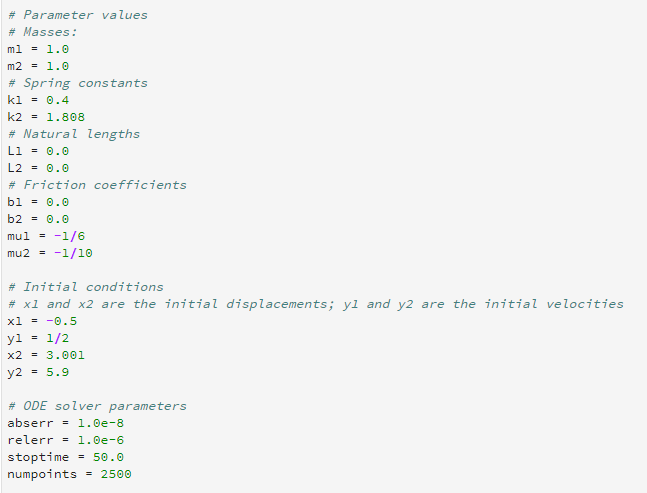
\includegraphics[width=0.6\textwidth]{Codigo5_1.PNG}
\end{figure}

Con lo que obtenemos las siguientes gráficas:
\begin{figure}[ht!]
\begin{subfigure}{0.6\textwidth}
  \centering
  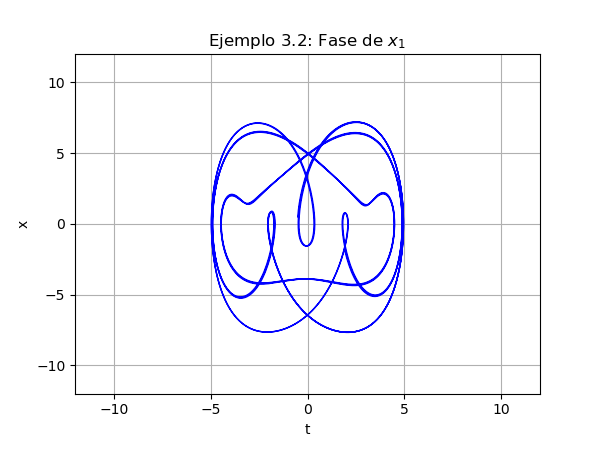
\includegraphics[width=0.75\linewidth]{ejemplo_3_2_2.png}
   \caption{Fase de $x_1$}
\end{subfigure}
\begin{subfigure}{0.6\textwidth}
  \centering
  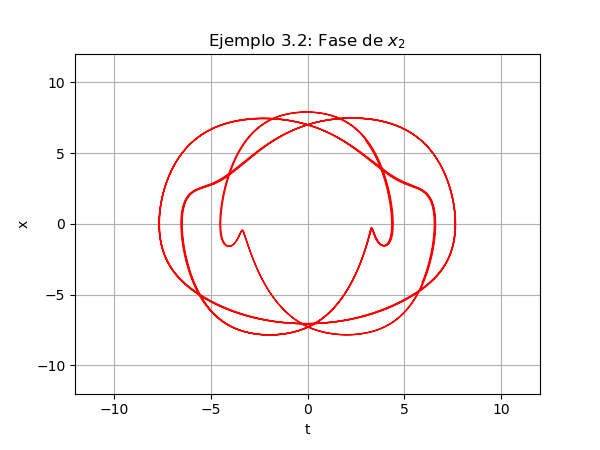
\includegraphics[width=0.75\linewidth]{ejemplo_3_2_3.png}
  \caption{Fase de $x_2$}
\end{subfigure}
\end{figure}
\begin{figure}[ht!]
 \centering
  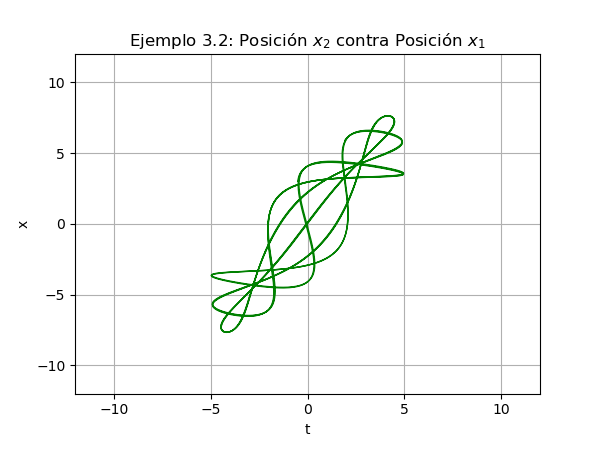
\includegraphics[width=0.6\textwidth]{ejemplo_3_2_1.png}
  \caption{Posición $X_2$ contra $x_1$}
\end{figure}

\pagebreak

\textbf{Ejemplo 3.3:} Asuma que $m_1 = m_2 = 1$. Describe el movimiento para las constantes de resorte $k_1 = 0.4$ y $k_2 = 1.808$, los coeficientes de amortiguamiento $\delta_1 = 0$ y $\delta_2 = 0$, coeficientes no lineales $\mu_1 = -1/6$ y $\mu_2 = -1/10$ con las condiciones iniciales ($x_1(0), \dot x_1(0), x_2(0), \dot x_2(0)) = (-0.6,1/2,3.001,5.9)$.

Agregando las condiciones iniciales y propiedades del sistema:
\begin{figure}[ht!]
 \centering
  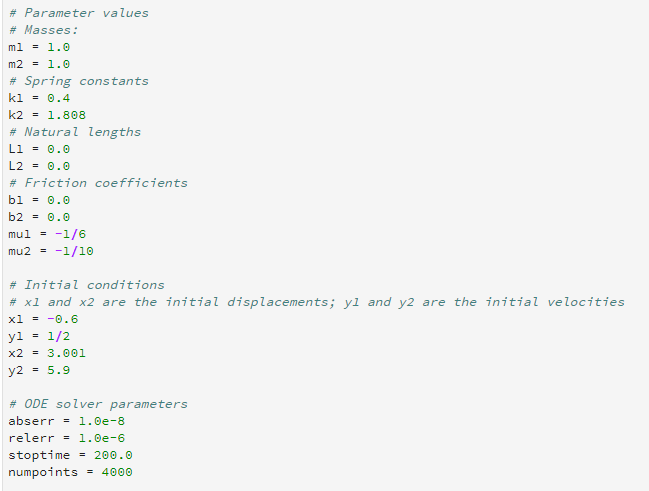
\includegraphics[width=0.6\textwidth]{Codigo5_2.PNG}
\end{figure}

Con lo que obtenemos las siguientes gráficas:
\begin{figure}[ht!]
\begin{subfigure}{0.6\textwidth}
  \centering
  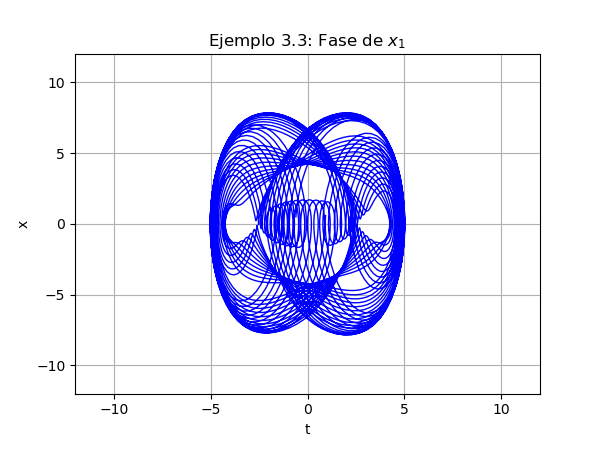
\includegraphics[width=0.75\linewidth]{ejemplo_3_3_2.png}
   \caption{Fase de $x_1$}
\end{subfigure}
\begin{subfigure}{0.6\textwidth}
  \centering
  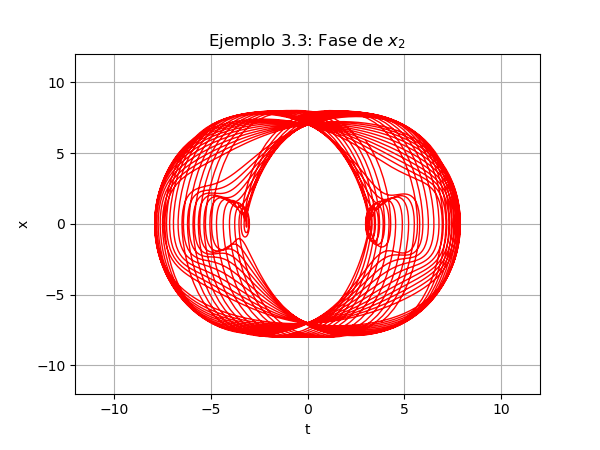
\includegraphics[width=0.75\linewidth]{ejemplo_3_3_3.png}
  \caption{Fase de $x_2$}
\end{subfigure}
\end{figure}
\begin{figure}[ht!]
 \centering
  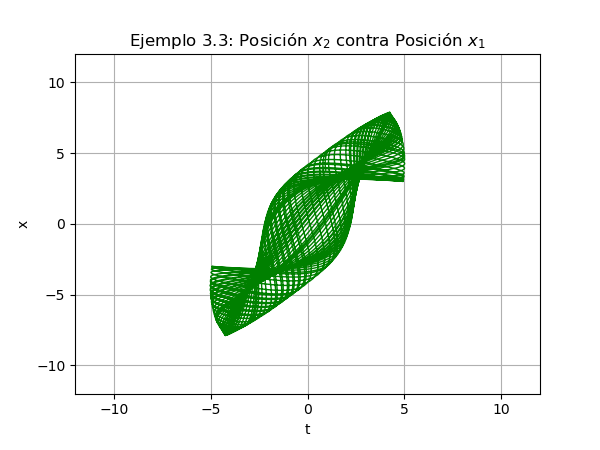
\includegraphics[width=0.6\textwidth]{ejemplo_3_3_1.png}
  \caption{Posición $x_2$ contra $x_1$}
\end{figure}

\subsection{Agregando Forzamiento}
Agregarle fuerza externa al modelo es muy simple, suponga que asumimos un forzamiento sinusoidal simple, de la forma $F cos(\omega t)$. Entonces el modelo queda:
\begin{center}
$m_1\ddot x_1 = - \delta_1\dot x_1 - k_1x_1 + \mu_1x_1^3 - k_2(x_1 - x_2) + \mu_2(x_1 - x_2)^3 + F_1cos\omega_1t$

$m_2 \ddot x_2 = - \delta\dot x_2 - k_2(x_2 - x_1) + \mu_2(x_2 - x_1)^3 + F_2cos\omega_2t$
\end{center}

Los rangos de movimiento para modelos no lineales con forzamiento son muy vastos, podemos encontrar resonancia no lineal, soluciones armónicas, soluciones armónicas y soluciones periódicas en estado estable. Las condiciones en las que esto ocurre no son fáciles de declarar.

\smallskip
\textbf{Ejemplo 4.1:} Asuma que $m_1 = m_2 = 1$. Describe el movimiento para las constantes de resorte $k_1 = 2/5$ y $k_2 =1$, los coeficientes de amortiguamiento $\delta_1 = 1/10$ y $\delta_2 = 1/5$, coeficientes no lineales $\mu_1 = 1/6$ y $\mu_2 = 1/10$, amplitudes de forzamiento $F_1 = 1/3$ y $F_2 = 1/5$, y frecuencias de forzamiento $\omega_1 = 1$ y $\omega_2 = 3/5$, con las condiciones iniciales ($x_1(0), \dot x_1(0), x_2(0), \dot x_2(0)) = (0.7,0,0.1,0)$.

Por el amortiguamiento, podemos esperar comportamientos diferentes con valores pequeños de tiempo y comportamientos de estado estable para valores grandes de tiempo. 
\smallskip

De nuevo, el código necesita modificarse para poder agregar el forzamiento. Después de los cambios, el código resulta así:

\begin{figure}[ht!]
 \centering
  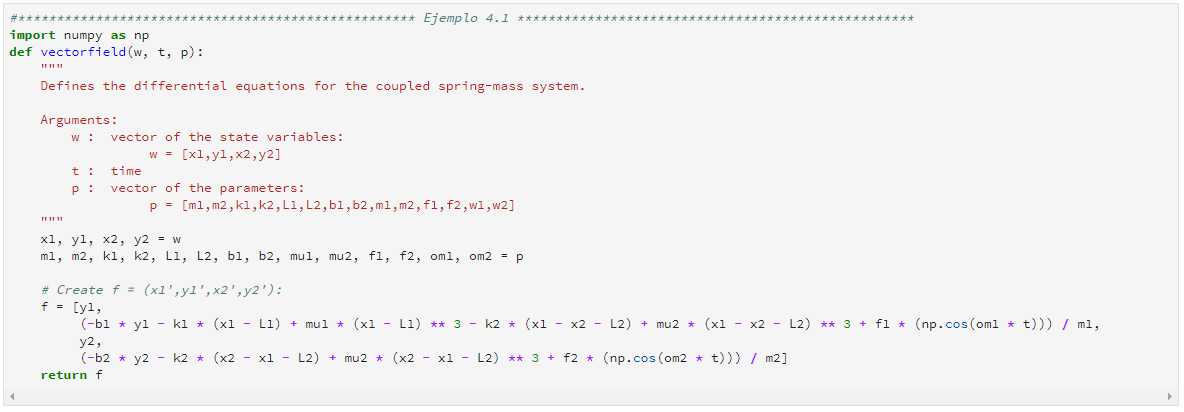
\includegraphics[width=0.65\textwidth]{Codigo6.PNG}
\end{figure}
\begin{figure}[ht!]
 \centering
  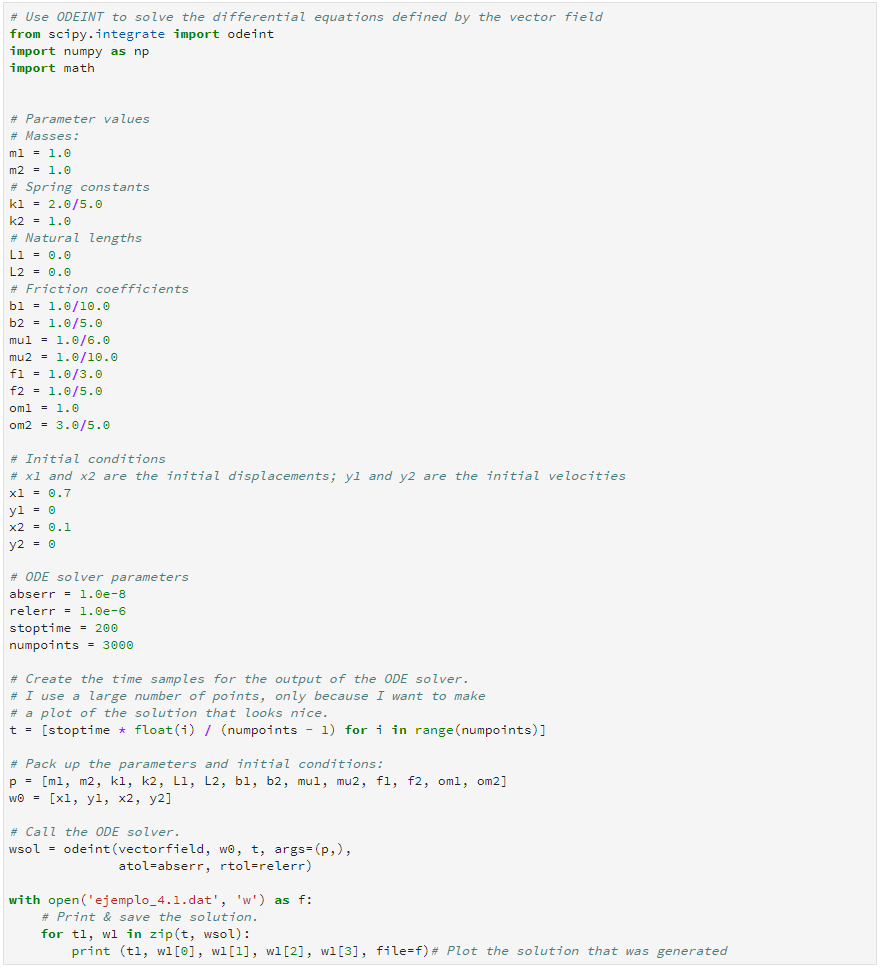
\includegraphics[width=0.65\textwidth]{Codigo7.png}
\end{figure}

Obteniendo las siguientes gráficas:

\begin{figure}[ht!]
\begin{subfigure}{0.6\textwidth}
  \centering
  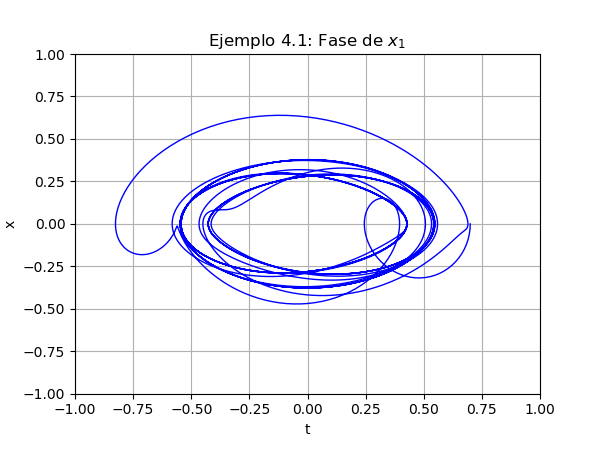
\includegraphics[width=\linewidth]{ejemplo_4_1_4.png}
   \caption{Fase de $x_1$}
\end{subfigure}
\begin{subfigure}{0.6\textwidth}
  \centering
  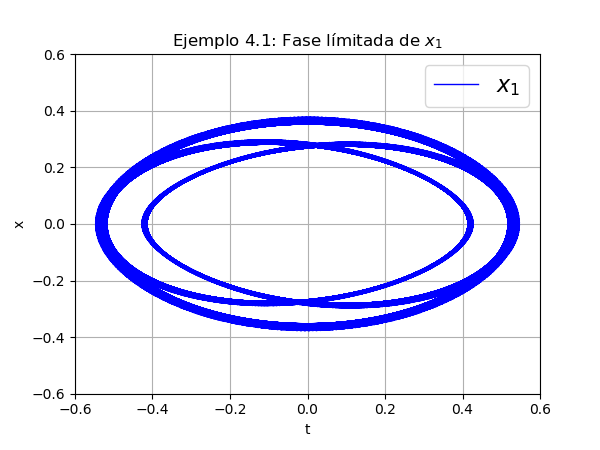
\includegraphics[width=\linewidth]{ejemplo_4_2_1.png}
  \caption{Ciclo limitado para $x_1$}
\end{subfigure}
\begin{subfigure}{0.6\textwidth}
  \centering
  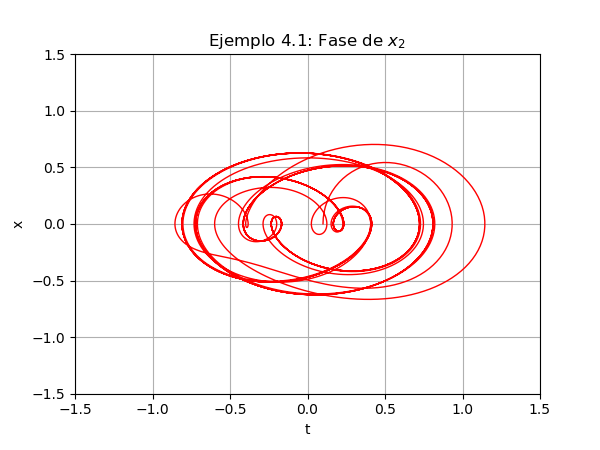
\includegraphics[width=\linewidth]{ejemplo_4_1_5.png}
  \caption{Fase de $x_2$}
\end{subfigure}
\begin{subfigure}{0.6\textwidth}
  \centering
  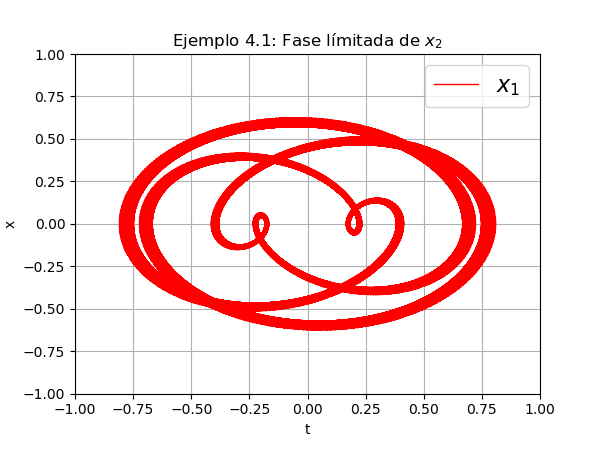
\includegraphics[width=\linewidth]{ejemplo_4_2_2.png}
  \caption{Ciclo limitado para $x_2$}
\end{subfigure}
\end{figure}
\begin{figure}[ht!]
\begin{subfigure}{0.6\textwidth}
  \centering
  \includegraphics[width=\linewidth]{ejemplo_4_1_2.png}
  \caption{Posición con respecto al tiempo de $x_1$}
\end{subfigure}
\begin{subfigure}{0.6\textwidth}
  \centering
  \includegraphics[width=\linewidth]{ejemplo_4_1_3.png}
  \caption{Posición con respecto al tiempo de $x_2$}
\end{subfigure}
\end{figure}

\begin{figure}[ht!]
\begin{subfigure}{0.6\textwidth}
  \centering
  \includegraphics[width=\linewidth]{ejemplo_4_1_1.png}
   \caption{Posición con respecto al tiempo de $x_1$ y $x_2$}
\end{subfigure}
\begin{subfigure}{0.6\textwidth}
  \centering
  \includegraphics[width=\linewidth]{ejemplo_4_1_6.png}
  \caption{Posición $x_2$ contra $x_1$}
\end{subfigure}
\end{figure}


\section{Conclusión}

Ha sido interesante continuar con el tema, ya que a diferencia de la actividad pasada, esta vez el tener que modificar el código para agregar las propiedades de oscilaciones no lineales y forzadas ha presentado un mayor reto. A pesar de esto, todo fue lograda con éxito, la parte de modificar el código fue lo único complicado, fuera de eso, el resto fue como seguir trabajando con la actividad pasada, lo que estuvo bien, por la poca disponibilidad de tiempo.  


Por otra parte, con esta actividad se puede reiterar en la opinión de que Jupyter Lab aporta un ambiente más agradable y cómodo que Jupyter Notebook, por sus múltiples y mejores herramientas.

\section{Bibliografía}
\begin{enumerate}
\item Fay, T., Graham, S. (2003) Coupled Srping Equations. Recuperado el 17 de Marzo del 2018 desde http://math.oregonstate.edu/~gibsonn/Teaching/MTH323\-010S15/Supplements/coupled\_spring.pdf

\end{enumerate}

\section{Apéndice}
\begin{enumerate}
\item \textbf{¿Qué más te llama la atención de la actividad completa? ¿Qué se te hizo menos interesante?}

Me gustó que hubo más interacción con el código, para adaptarlo para que pudiera graficar correctamente los ejemplos del artículo. Ésta y la actividad pasada han sido muy entretenidas, ya que es interesante ver temas vistos en cursos pasados ser aplicados a la programación.

\item \textbf{¿De un sistema de masas acopladas como se trabaja en esta actividad, hubieras pensado que abre toda una nueva área de fenómenos no lineales?}

Alguna vez fue mencionado por el profesor en el curso de Mecánica II, pero nunca supe cómo eran o funcionaban, hasta ahora; pero fuera de eso, yo no conocía su existencia. 

\item \textbf{¿Qué propondrías para mejorar esta actividad? ¿Te ha parecido interesante este reto?} 

La actividad así como tal, estuvo muy bien, ya que no tomó tanto tiempo y fue como continuar con la actividad pasada, pero un nivel más arriba.

\item \textbf{¿Quisieras estudiar mas este tipo de fenómenos no lineales?}

Sí, ha sido muy interesante ver estos temas, además de que pienso que son herramientas muy útiles, no solo para el curso, si no para cualquier área de la física. 

\end{enumerate}

\end{center}

\end{document}